% Created: 2019-12-10
% Plot participant data
% http://github.com/zhaobn/magic_stones

\documentclass{article}
\title{[Magic Stones] Plots for Experiment 1}
\author{Bonan Zhao (b.zhao@ed.ac.uk)}

% Text formats: margin, font, spacing
\usepackage[margin=0.8in]{geometry}
\usepackage{charter}
\renewcommand{\baselinestretch}{1.3}

% Graphics
\usepackage{graphicx}
\usepackage{subcaption}
\graphicspath{{../figs/}}


\begin{document}
\maketitle


\begin{figure}[h!]
	\centering
  \begin{subfigure}[t]{0.31\textwidth}
  	\centering
  	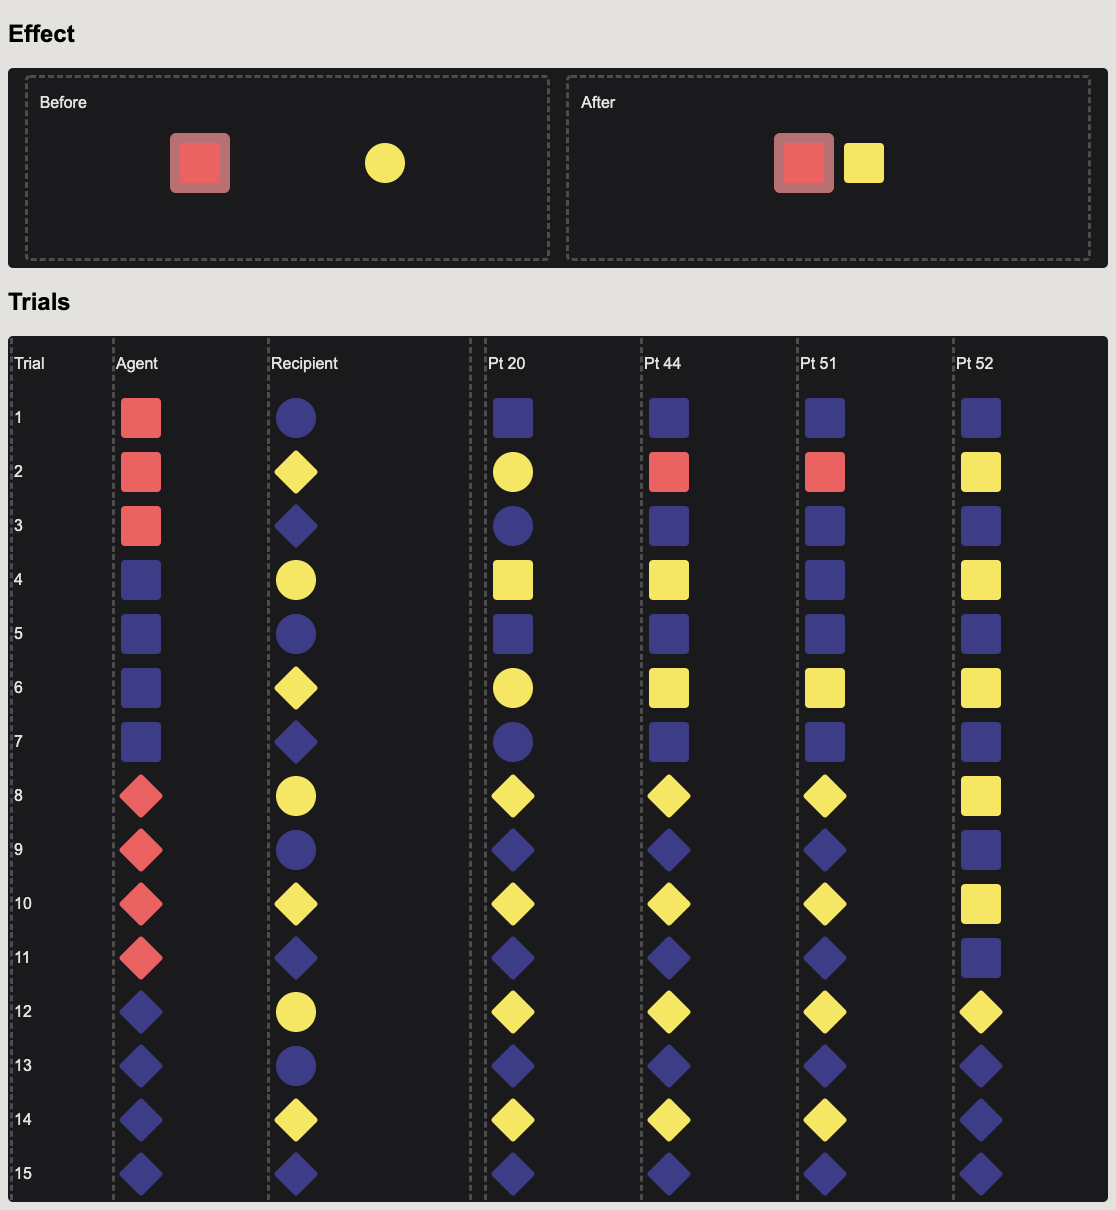
\includegraphics[width=\linewidth]{raw_g1} 
  	\caption{To the same shape} \label{fig:raw_g1}
  \end{subfigure}
  \hfill
  \begin{subfigure}[t]{0.31\textwidth}
  	\centering
  	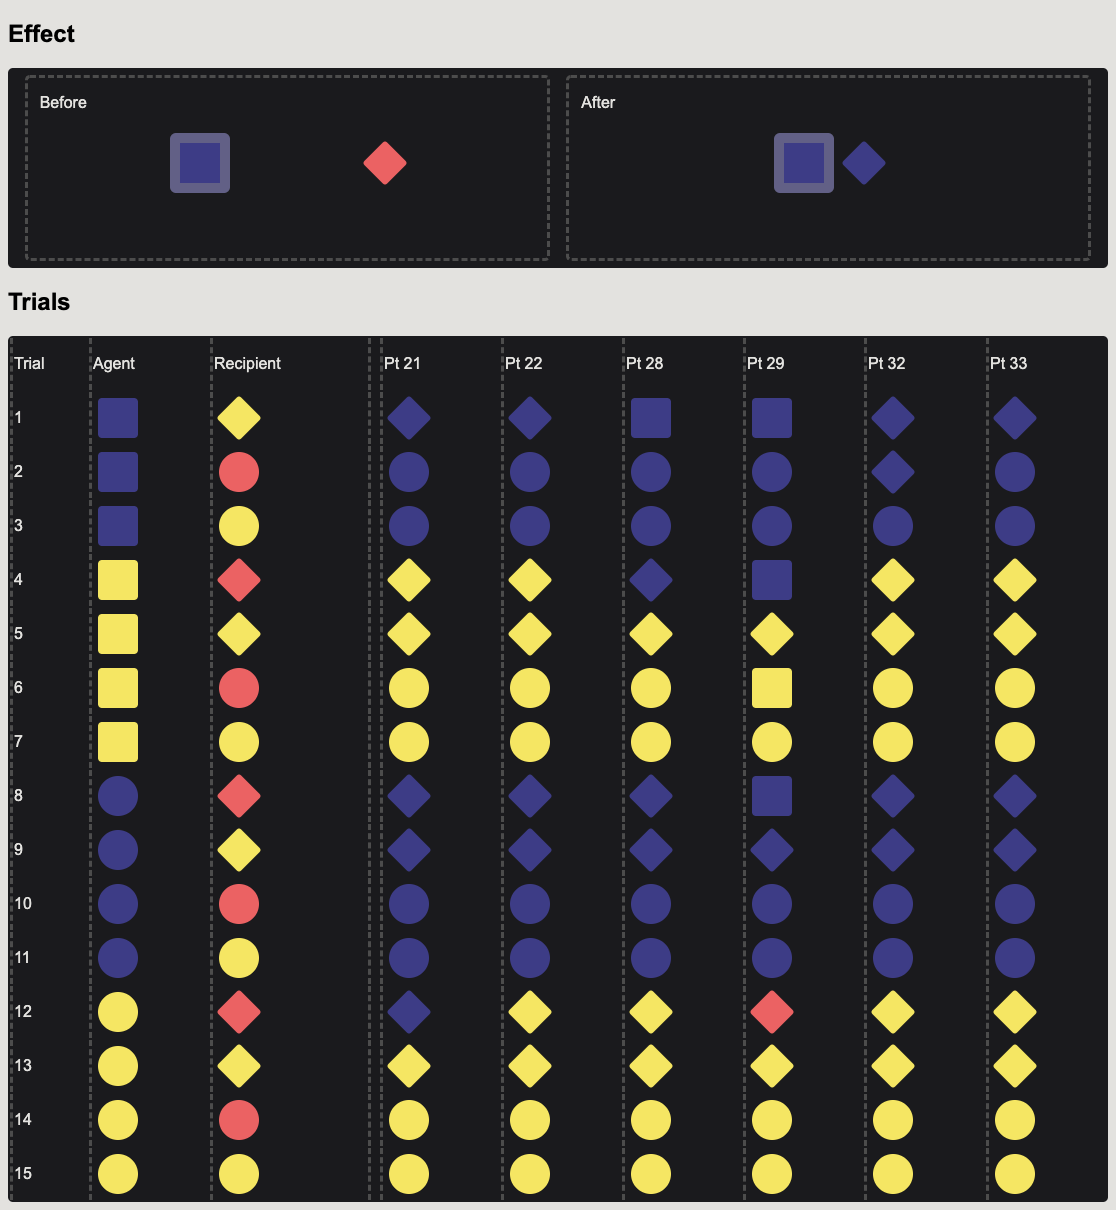
\includegraphics[width=\linewidth]{raw_g3} 
  	\caption{To the same color} \label{fig:raw_g3}
  \end{subfigure}
  \hfill
  \begin{subfigure}[t]{0.31\textwidth}
  	\centering
  	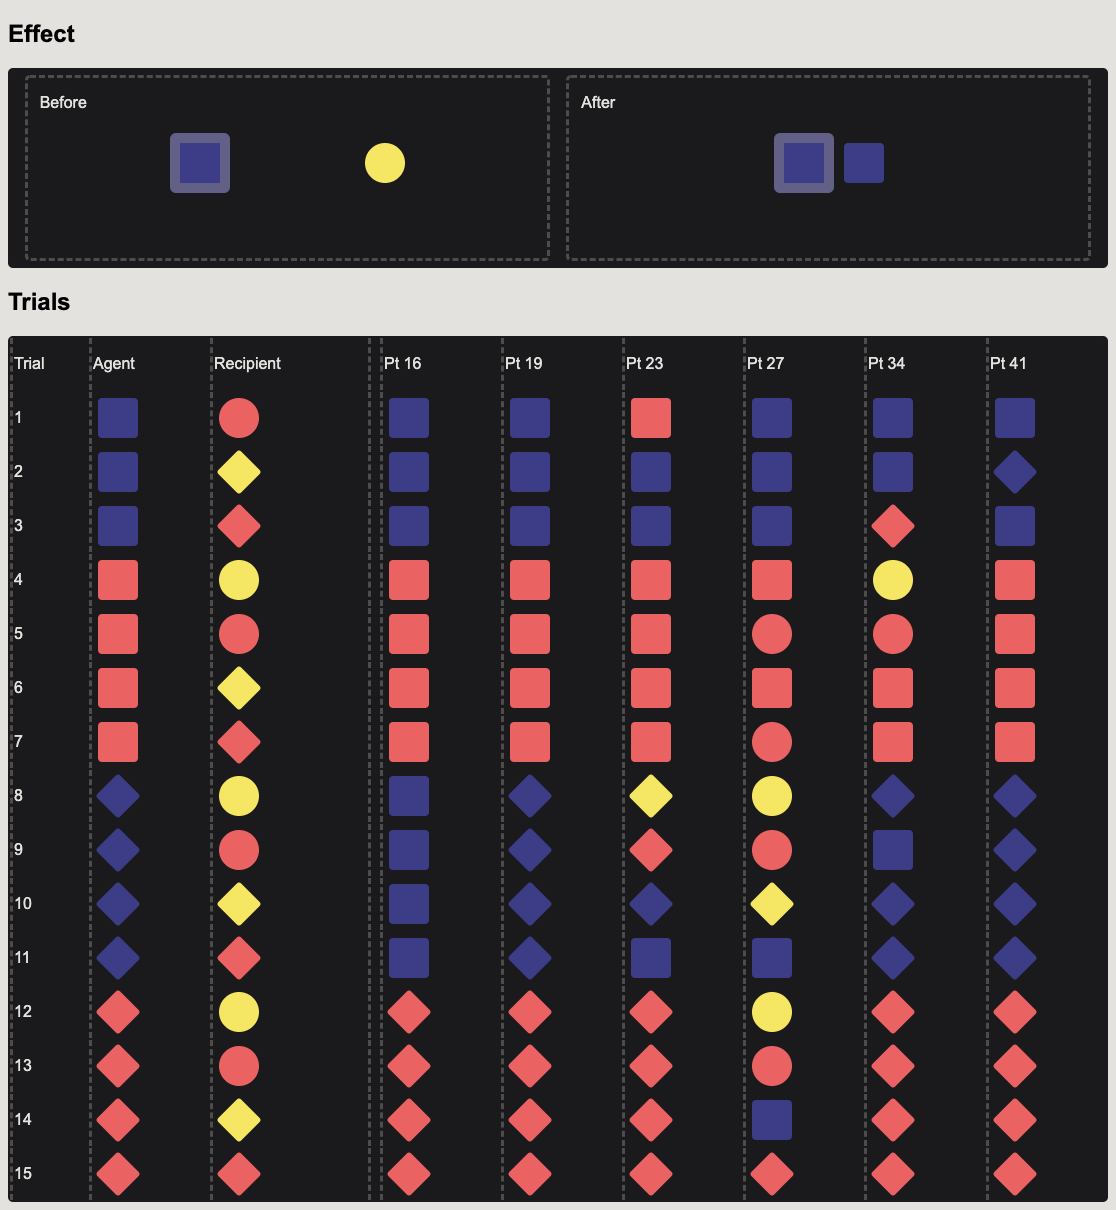
\includegraphics[width=\linewidth]{raw_g6} 
  	\caption{To the same object} \label{fig:raw_g6}
  \end{subfigure}

  \vspace{1em}
  \begin{subfigure}[t]{0.31\textwidth}
  	\centering
  	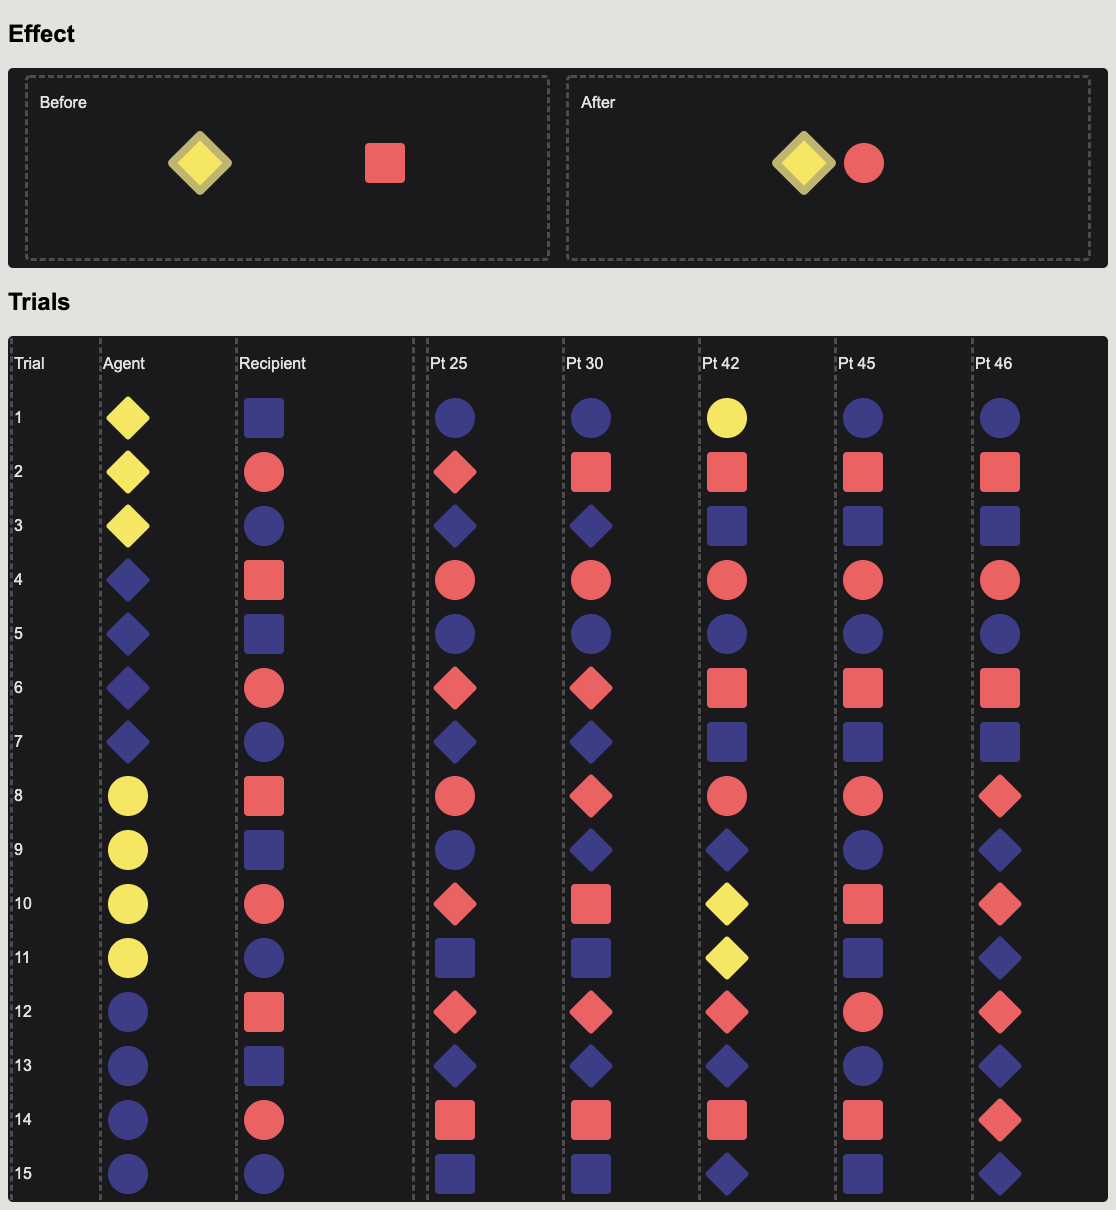
\includegraphics[width=\linewidth]{raw_g2} 
  	\caption{To a different shape} \label{fig:raw_g2}
  \end{subfigure}
  \hfill
  \begin{subfigure}[t]{0.31\textwidth}
  	\centering
  	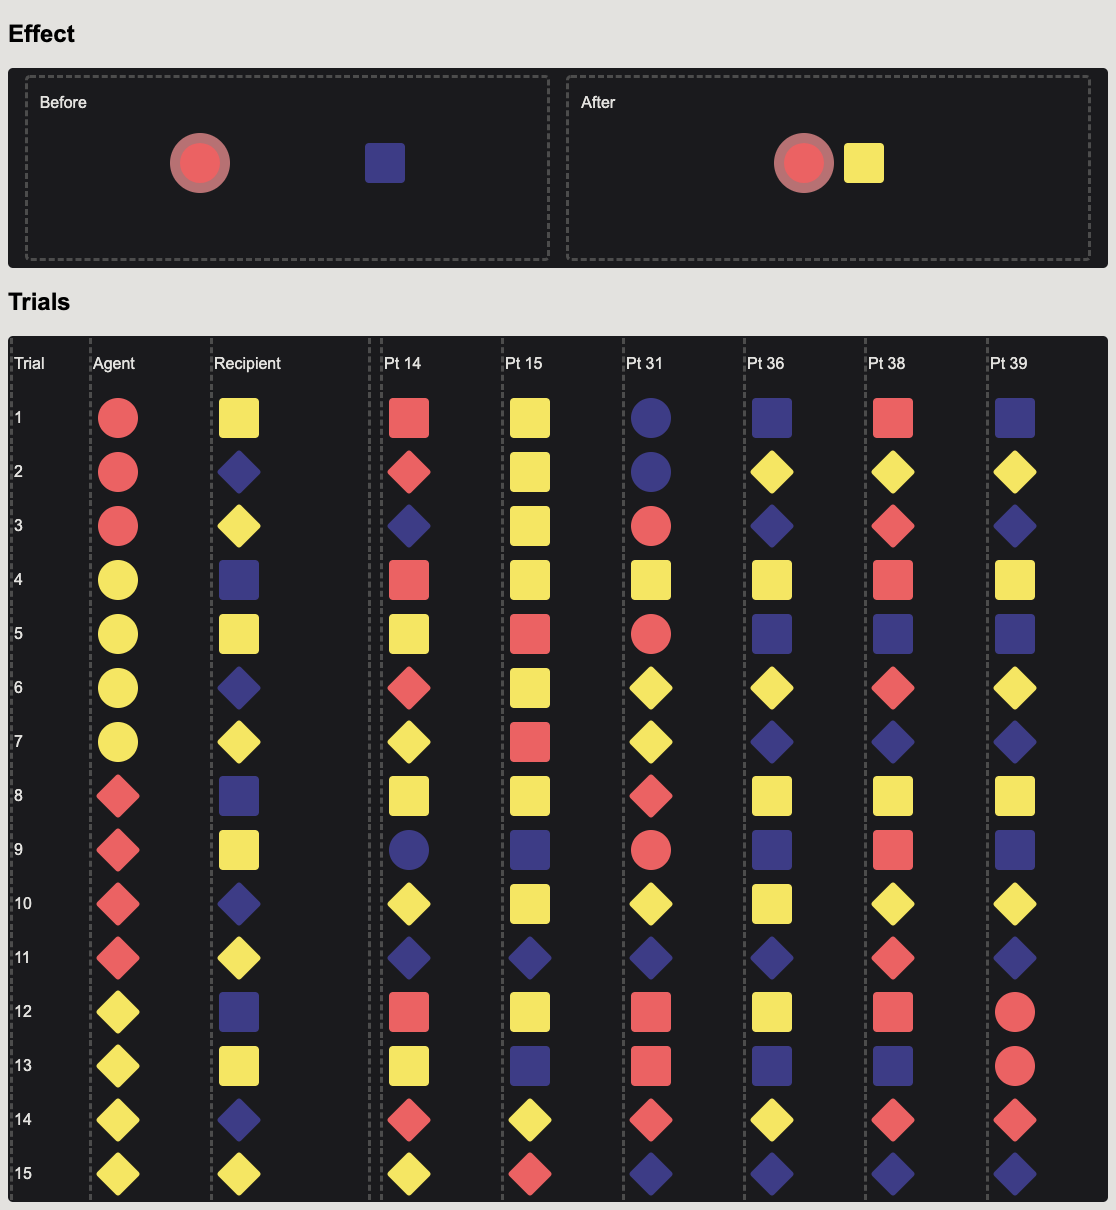
\includegraphics[width=\linewidth]{raw_g4} 
  	\caption{To a different color} \label{fig:raw_g4}
  \end{subfigure}
  \hfill
  \begin{subfigure}[t]{0.31\textwidth}
  	\centering
  	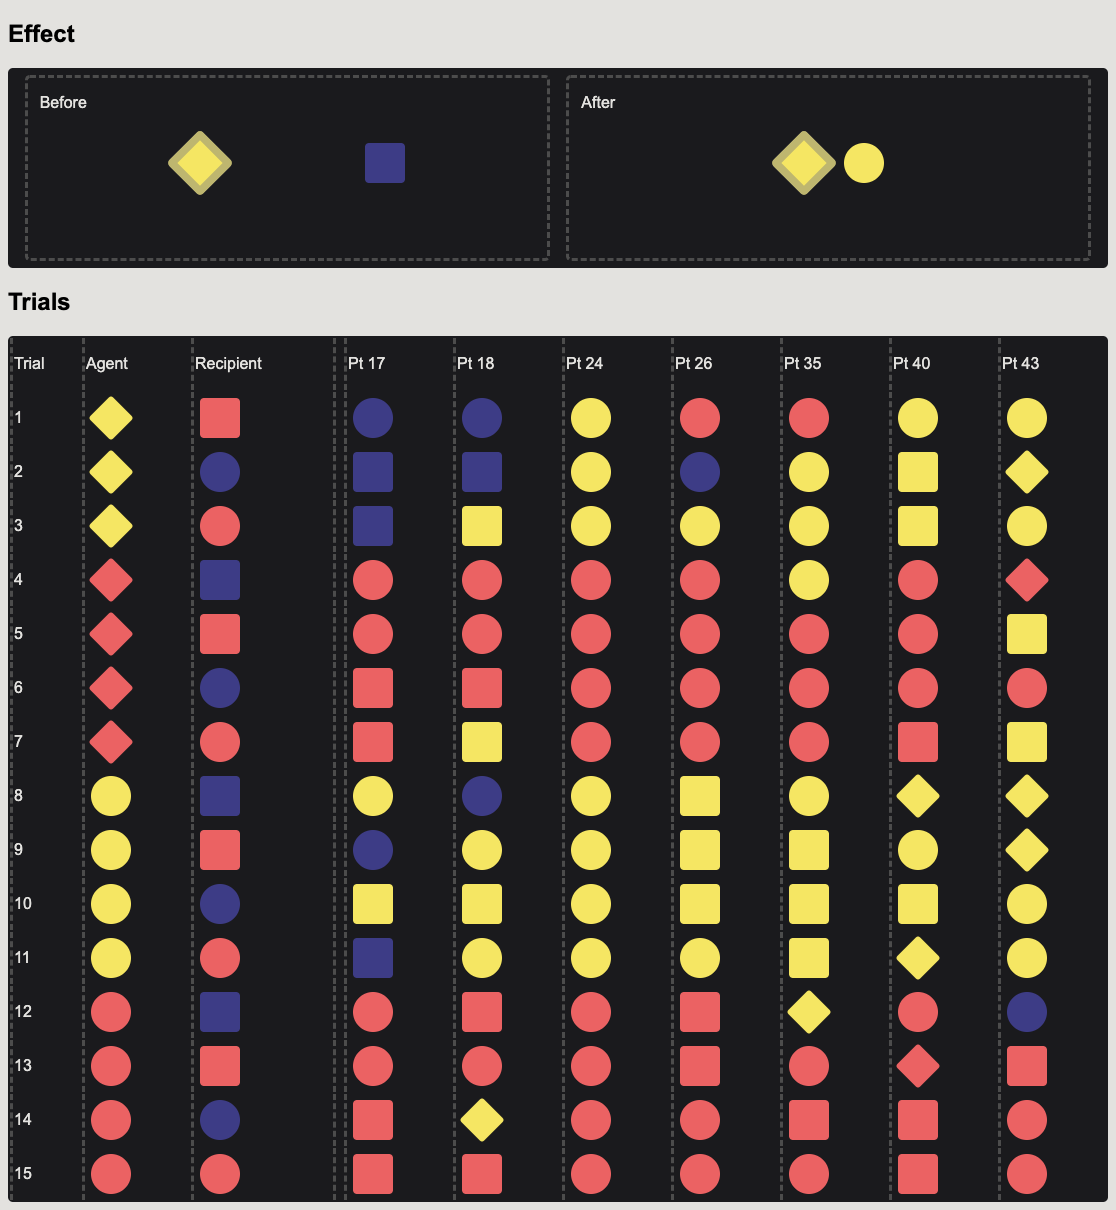
\includegraphics[width=\linewidth]{raw_g5} 
  	\caption{To a different object} \label{fig:raw_g5}
  \end{subfigure}
  \caption{Participant data per group per trial. Each figure is for one group - at the top is a summary of the magic effect participants watched, and below is a complete visualization of participant selections. In the selection part, each row is for one trial: the first two icons are the magic stone and normal stone that a participant is asked to make a prediction for, and the rest are participant selections.}
  % \caption{Some general caption of all the figures. In (\subref{fig:group01}) you can see a  green square....}
\end{figure}

\newpage
\begin{figure}
  \centering
  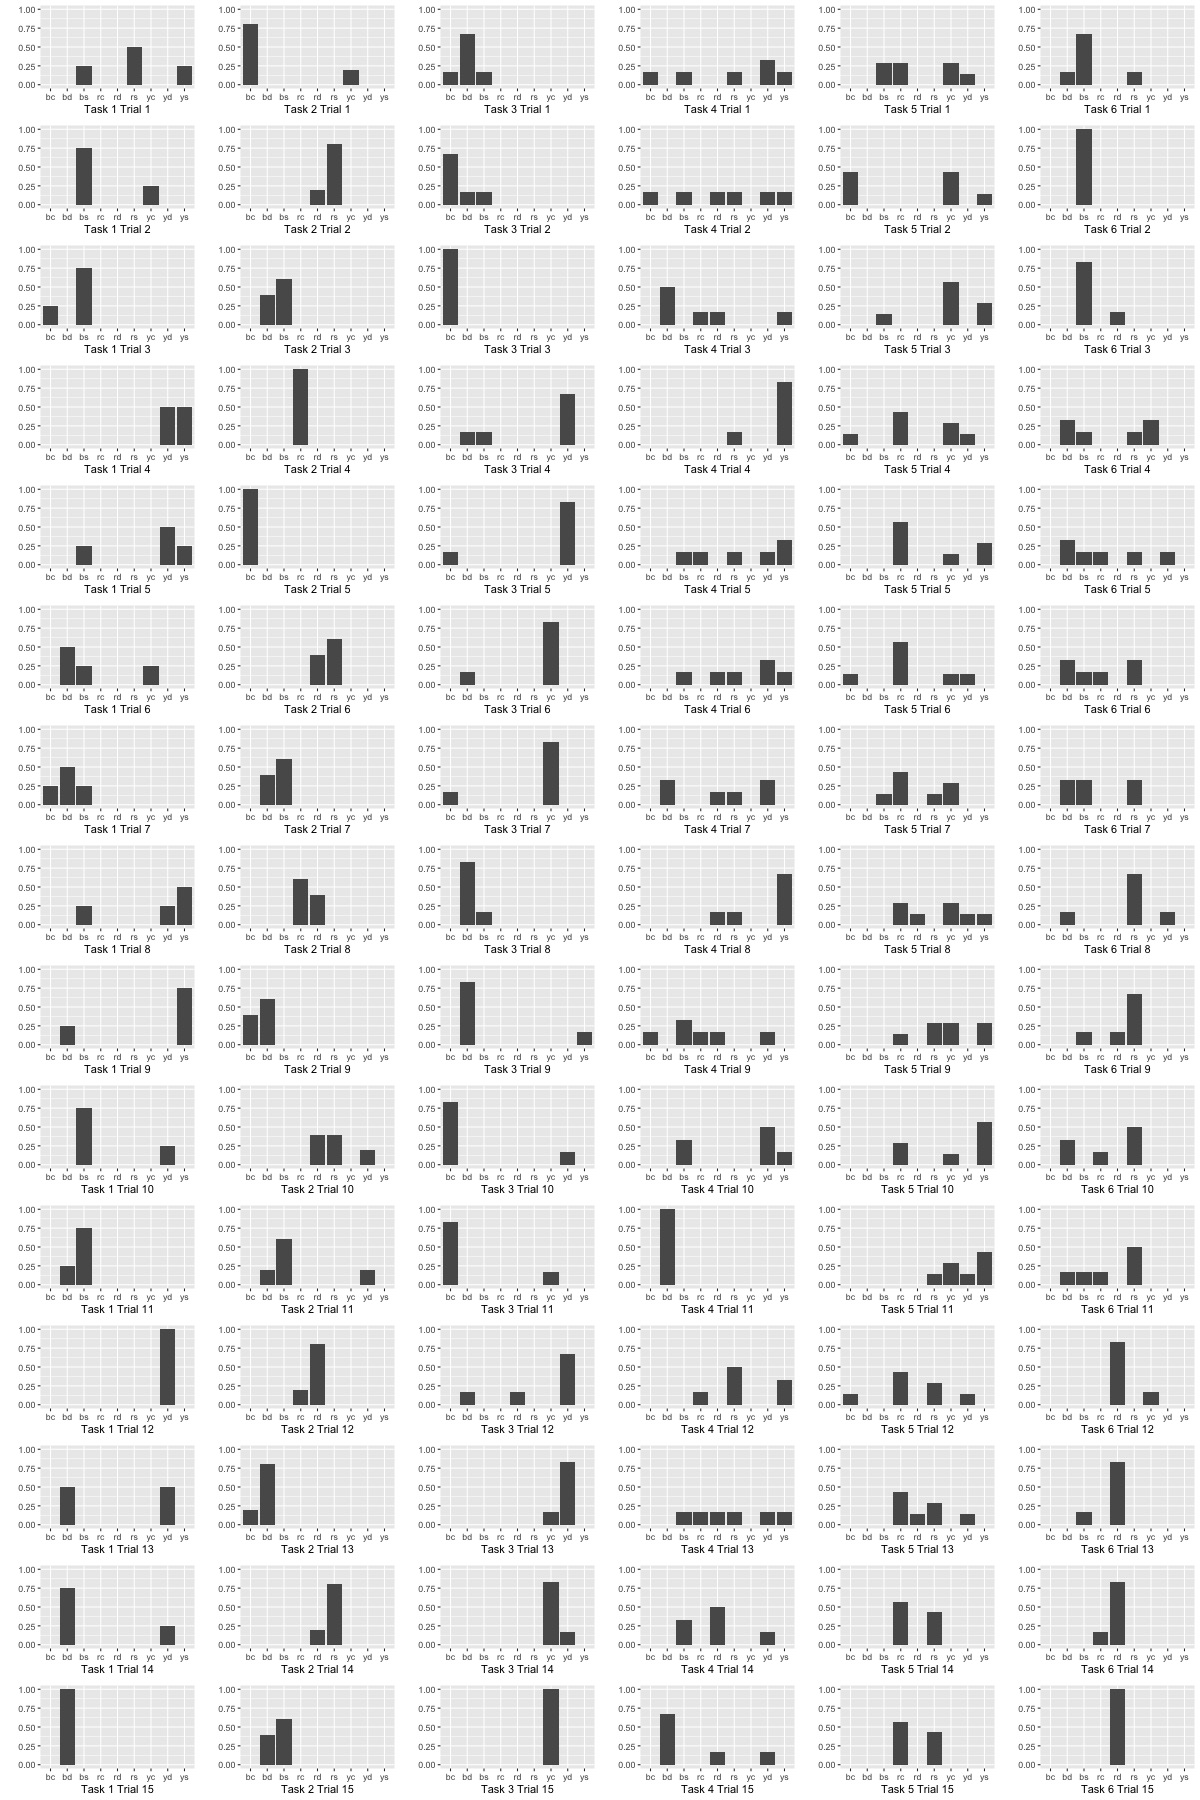
\includegraphics[width=.85\linewidth]{trials}
  \caption{Participant raw selections summary. Each row is for one trial, and each column is for one task. For each sub-figure, y-axis is percentage, and x-axis from left to right is: bc, bd, bs, rc, rd, rs, yc, yd, ys.}
\end{figure}

\newpage
\begin{figure}
  \centering
  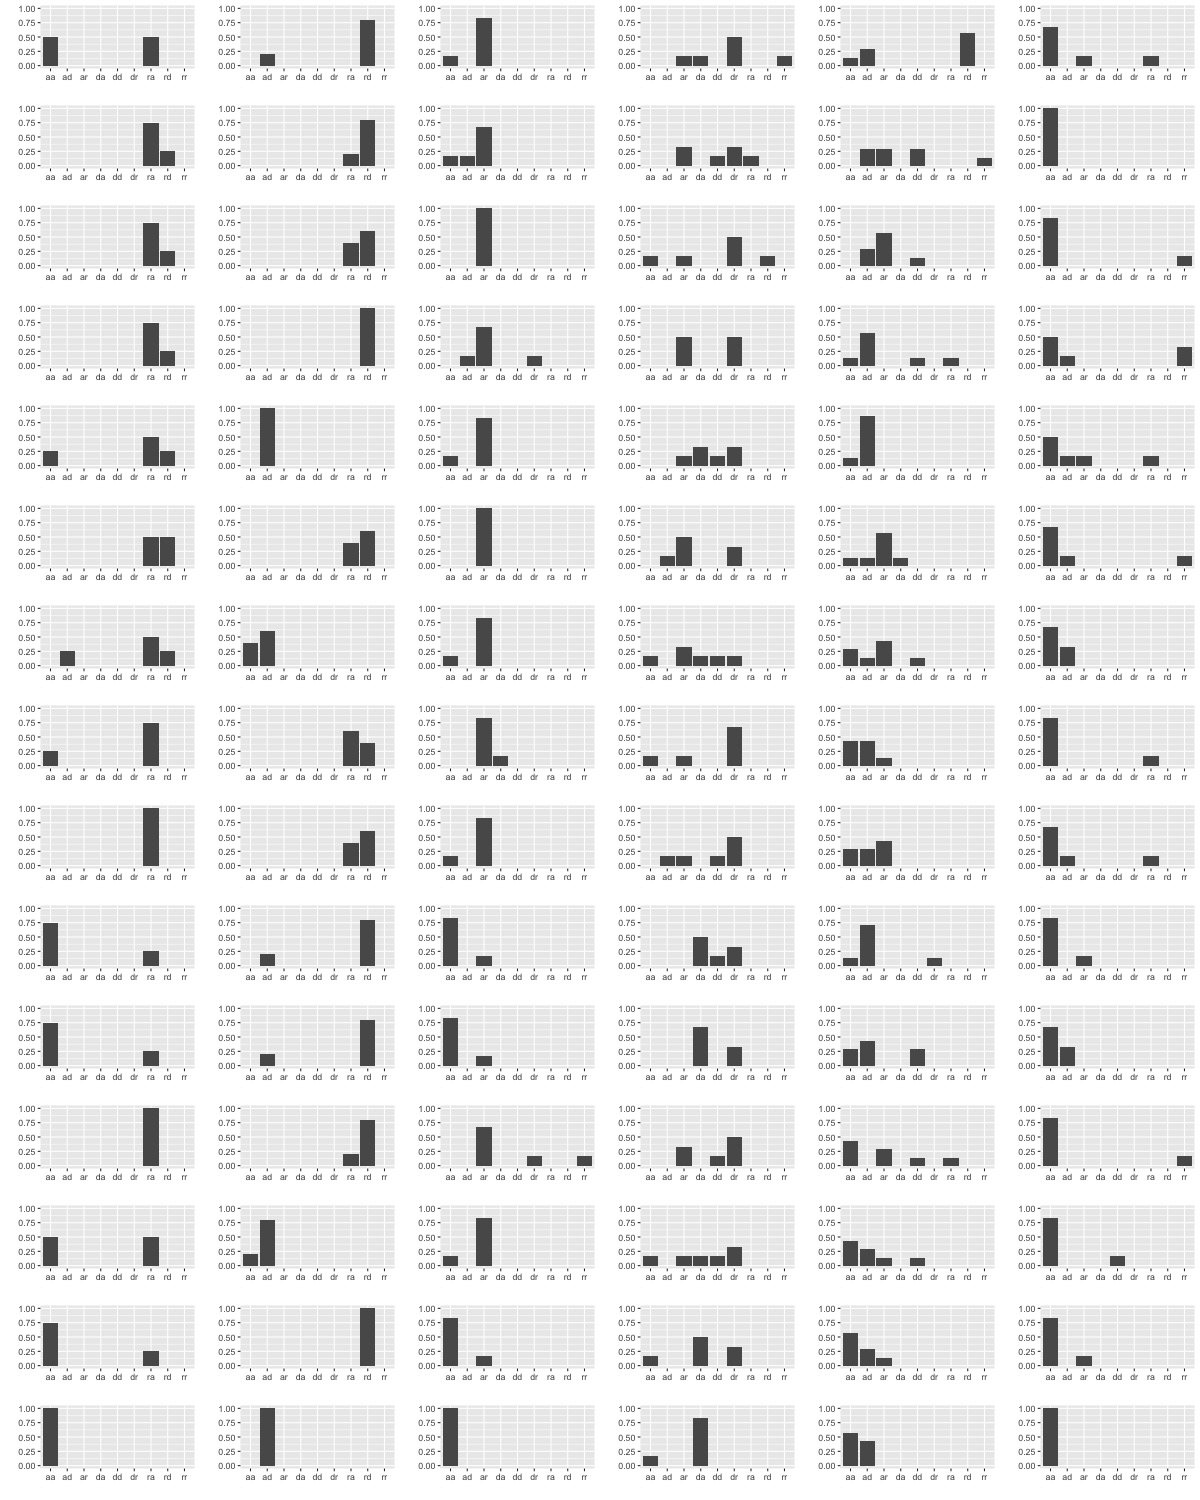
\includegraphics[width=.85\linewidth]{trials_relative}
  \caption{Relative selections summary. Each row is for one trial, and each column is for one task. For each sub-figure, y-axis is percentage, and x-axis from left to right is: aa, ad, ar, da, dd, dr, ra, rd, rr.}
\end{figure}

\newpage
\begin{figure}
  \centering
  \begin{subfigure}[t]{0.25\textwidth}
    \centering
    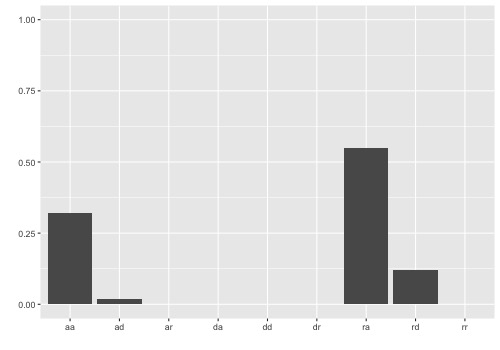
\includegraphics[width=\linewidth]{agg_g1} 
    \caption{To the same shape} \label{fig:agg_g1}
  \end{subfigure}
  \begin{subfigure}[t]{0.25\textwidth}
    \centering
    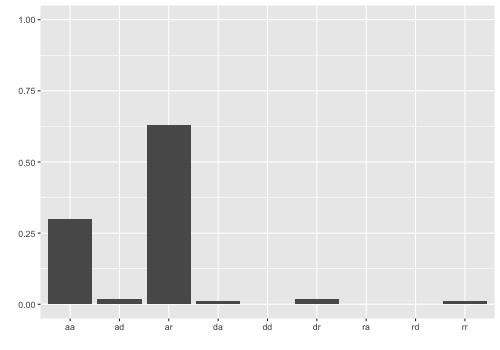
\includegraphics[width=\linewidth]{agg_g3} 
    \caption{To the same color} \label{fig:agg_g3}
  \end{subfigure}
  \begin{subfigure}[t]{0.25\textwidth}
    \centering
    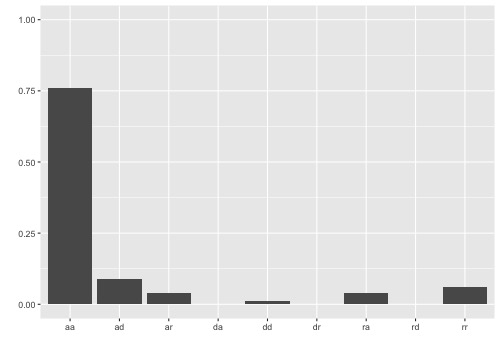
\includegraphics[width=\linewidth]{agg_g6} 
    \caption{To the same object} \label{fig:agg_g6}
  \end{subfigure}

  \vspace{1em}
  \begin{subfigure}[t]{0.25\textwidth}
    \centering
    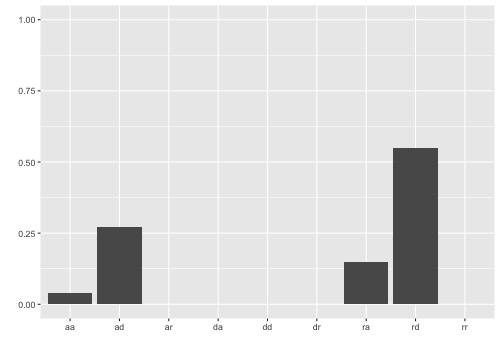
\includegraphics[width=\linewidth]{agg_g2} 
    \caption{To a different shape} \label{fig:agg_g2}
  \end{subfigure}
  \begin{subfigure}[t]{0.25\textwidth}
    \centering
    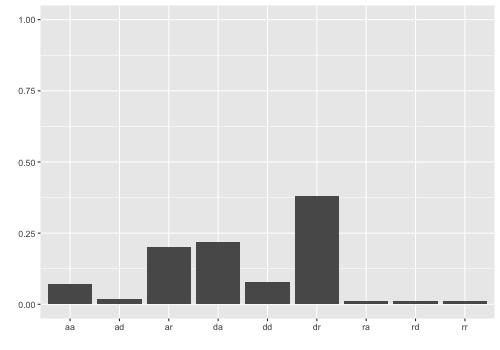
\includegraphics[width=\linewidth]{agg_g4} 
    \caption{To a different color} \label{fig:agg_g4}
  \end{subfigure}
  \begin{subfigure}[t]{0.25\textwidth}
    \centering
    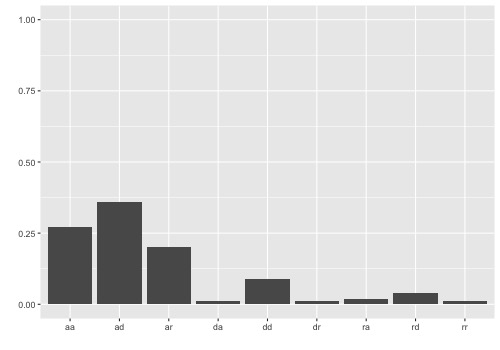
\includegraphics[width=\linewidth]{agg_g5} 
    \caption{To a different object} \label{fig:agg_g5}
  \end{subfigure}
  \caption{Aggregated relative selections per task. For each sub-figure, y-axis is percentage, and x-axis from left to right is: aa, ad, ar, da, dd, dr, ra, rd, rr.}
\end{figure}

\begin{figure}
  \centering
  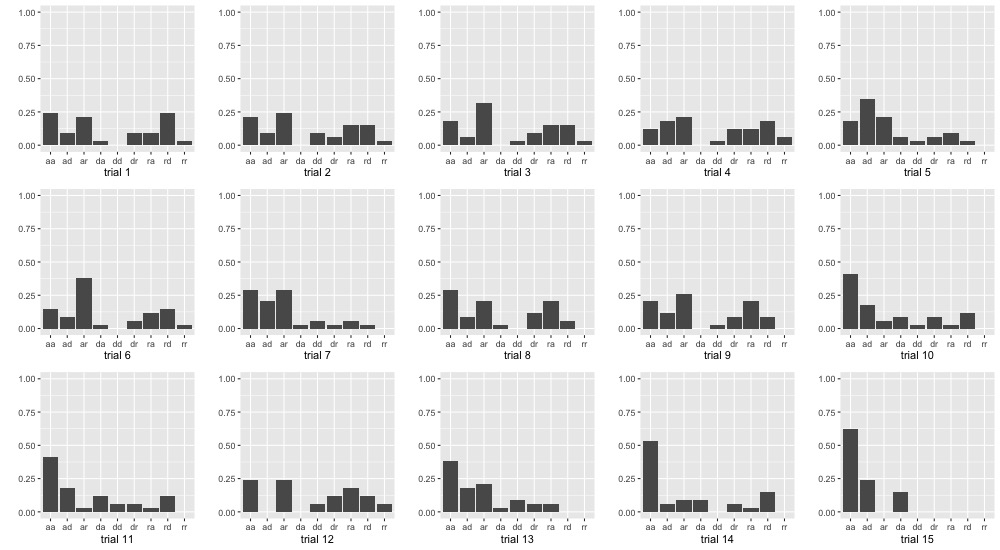
\includegraphics[width=\linewidth]{agg_trials}
  \caption{Aggregated relative selections per trial. For each sub-figure, y-axis is percentage, and x-axis from left to right is: aa, ad, ar, da, dd, dr, ra, rd, rr.}
\end{figure}


\end{document}